\chapter{Budowa programu}
W rozdziale trzecim zawarto informacje dotyczące budowy programu. Na początku opisana jest jego struktura w postaci diagramów. Następnie opisane są poszczególne fragmenty programu. Na końcu znajduje się opis interfejsu graficznego programu.


\section{Struktura programu}

Poniżej znajduje się opis struktury plików oraz opis zawartości poszczególnych katalogów programu.

\begin{itemize}
	\item \textbf{photo-2-midi.py} - interfejs programu, uruchamia program.
	\item \textbf{convert\_to\_MIDI.py} - główna część programu, zarządza działaniem procesu uzyskiwania informacji ze zdjęć.
	\item \textbf{staff\_detection.py} - w skład tego pliku wchodzą funkcje odpowiedzialne za detekcję pięciolinii.
	\item \textbf{dewarp\_page.py} - plik zawierający całą logikę i działanie części programu odpowiedzialnej za usuwanie wypaczenia z obrazów wejściowych.
	\item \textbf{image\_segmentation.py} - jest plikiem posiadającym wszystkie funkcje mające za zadanie poprawne podzielenie obrazu na mniejsze fragmenty nadające się na przekazanie dla wytrenowanego modelu uczenia maszynowego.
	\item \textbf{utils.py} - przechowuje funkcje dodatkowe.
	\item \textbf{trained\_model} - folder zawierający wytrenowany model uczenia maszynowego.
	\item \textbf{ML\_model/model} - folder przechowujące niezbędne pliki do użycia wytrenowanego modelu uczenia głębokiego.
\end{itemize}

\section{Diagram maszyny stanowej}

\begin{figure}
	\centering
	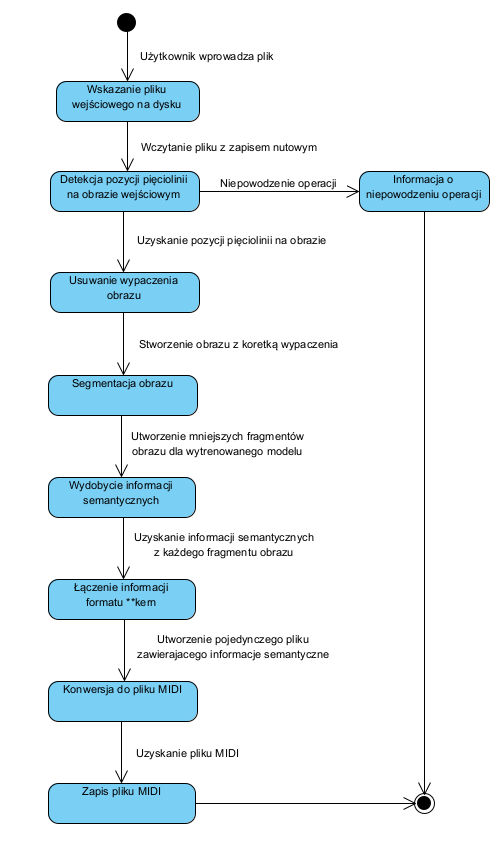
\includegraphics[width=10cm]{images/diagram-maszyny-stanowej-programu.png}
	\caption{Diagram maszyny stanowej programu.}
	\label{fig:program-state-machine}
\end{figure}


\section{Interfejs graficzny}

Interfejs został stworzony przy użyciu biblioteki \textit{PySimpleGUI}.

\begin{figure}[h]
	\centering
	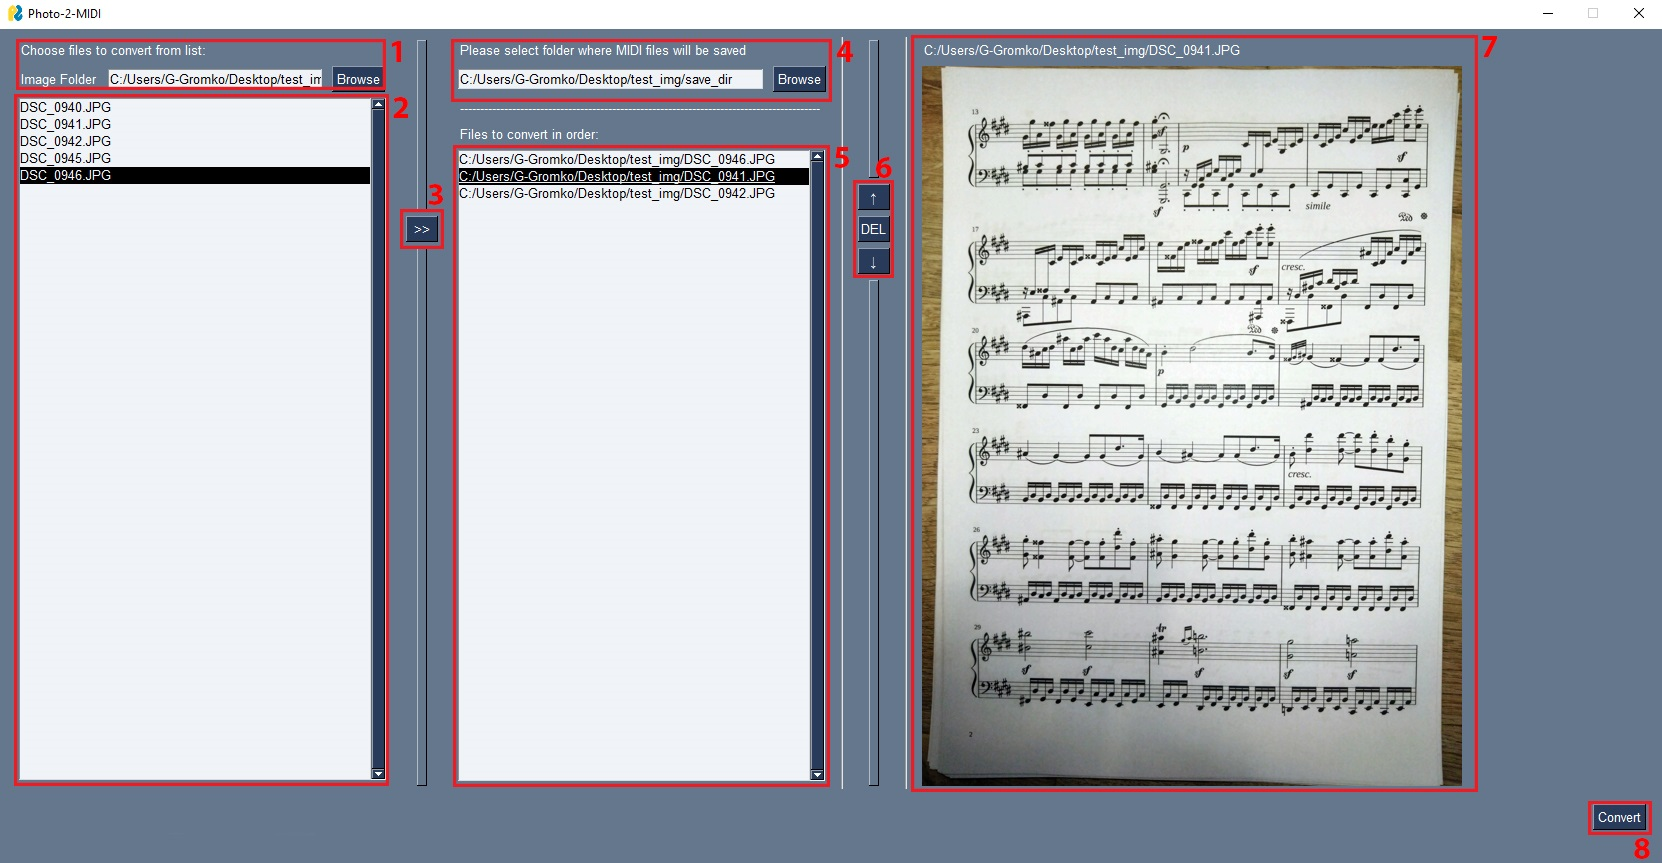
\includegraphics[width=16cm]{images/gui}
	\caption{Interfejs graficzny programu Photo-2-MIDI}
	\label{fig:gui}
\end{figure}

\begin{enumerate}
	\item Pole tekstowe do wprowadzenia ścieżki folderu ze zdjęciami zapisu nutowego.
	\item Lista plików w wybranym folderze.
	\item Przycisk do przeniesienia zaznaczonego pliku do listy plików do konwersji.
	\item Pole tekstowe do wprowadzenia ścieżki folderu do którego mają zostać zapisane uzyskane pliki MIDI.
	\item Lista plików przeznaczonym do konwersji, ułożone w kolejności w której konwersja ma się odbyć.
	\item Przyciski do organizacji plików przeznaczonych do konwersji, kolejno: przesuń wybrany plik w górę na liście, usuń wybrany plik z listy, przesuń wybrany plik w dół na liście.
	\item Podgląd wybranego pliku z jednej z list.
	\item Przycisk uruchamiający konwersję zdjęć do plików MIDI.
\end{enumerate}